\documentclass[final,a4paper]{article}
\usepackage[utf8]{inputenc}
\usepackage{amsmath}
\usepackage{graphicx}
\usepackage{url}
\usepackage{fancyhdr}
\usepackage{datetime}
\usepackage{titlesec}
\usepackage{float}

\setlength{\parindent}{0em}
\setlength{\parskip}{1em}

\titlespacing\section{0pt}{1.5em}{-0.5em}
\titlespacing\subsection{0pt}{1.0em}{-0.5em}
\titlespacing\subsubsection{0pt}{0.5em}{-1.0em}

\newcommand{\course}{Operating Systems, 5dv171}
\newcommand{\semester}{Fall 2017}
\newcommand{\assignment}{Project: Writing a Linux kernel module}
\newcommand{\authors}{
  Igor Ramazanov, ens17irv@cs.umu.se\\
  Erik Ramos, c03ers@cs.umu.se\\
  Bastien Harendarczyk, ens17bhk@cs.umu.se\\
  \vspace{1em}
}
\newcommand{\lecturer}{Jan Erik Moström}
\newcommand{\assistants}{Adam Dahlgren}
\newcommand{\codebase}{https://git.cs.umu.se/c03ers/5dv171-project}

\title{
  \pagenumbering{gobble}
  \begin{center}
  \vspace{4em}
  {\LARGE \bf \course{}, \semester}\\
  {\Large \bf \assignment}\\
  \vspace{4em}
  {\normalsize
  {\bf Teacher}\\
  {\lecturer}\vspace{1em}\\
  {\bf Teaching assistant}\\
  {\assistants}\vspace{1em}\\
  {\bf Group members}\\
  \authors
  {\bf Gitlab repository}\vspace{-1em}\\
  {\codebase}}
  \end{center}
  \vspace{2em}
}

\author{}
\date{}
\pagestyle{fancy}
\fancyhead{}
\fancyhead[R]{\footnotesize \the\year-\twodigit{\the\month}-\twodigit{\the\day}}
\renewcommand{\headrulewidth}{0em}

\begin{document}
\maketitle
  \begin{center}
  {\bf Abstract }\\
  \vspace{0.5em}
  \begin{tabular}{ p{25em} }
  \hline
  \vspace{0.0em}
  The project described in this report implements a Linux kernel module
  which provides a key-value storage, that can be used by different programs
  to exchange data and store it between program executions and module
  installations.\vspace{0.7em}\\
  \end{tabular}
  \end{center}
\pagebreak
\tableofcontents
\newpage
\pagenumbering{arabic}
\section{Problem description}
The goal with this project was to write a Linux Kernel Module (LKM) that allowed
different processes running on the same Linux machine, to access shared data
through key-value mappings stored in the kernel. The system had to be robust
enough to allow multiple processes, running on multiple processors, to use it
without accidentally corrupting the stored data. Additionally, the module
needed to store the data in such a way that it could be recovered, even if the
module was re-installed.

A user-space application also had to be implemented, in order  to demonstrate
the functionality of the LKM. To measure the performance of the module, a
benchmark program was also necessary.

\section{User's guide}
The project consists of three parts - the kernel module, a user-space
test program and a benchmark program to test the performance of the kernel
module. All files required to build these parts can be found in the gitlab
repository.

To download the project, begin by cloning the repository typing the following in
a terminal:
\begin{center}
{\tt git clone \codebase}
\end{center}

Each part is assigned to a separate directory; \texttt{module} for the kernel
module, \texttt{program} for the user-space program and \texttt{benchmark}
for the benchmark program. Each of these directories contain their own
make-files, so building any of the parts can be done by typing
\texttt{make} in the terminal, from the respective directory.

Once built, a super-user may install the module by typing 
{\tt insmod shared\_map.ko} in the terminal, while in the module directory.
Running {\tt rmmod shared\_map } will remove the module.

The test program \emph{test}, can be used both for putting data
into the module and to retrieve data from it. Inserting data is done like this:
\begin{center}
{\tt ./test set key value}
\end{center}
To retrieve data from the module using the test program, instead write this:
\begin{center}
{\tt ./test get key}
\end{center}

Data entered into the module is saved as files in
\begin{center}
{\texttt{/var/tmp/shared\_map/}}
\end{center}
and will remain on the hard-disk even after removing the module. Re-installing
the module will recover data from previous installations.

After the module has been installed, the benchmark program can be used to
measure its performance. To run it, go to the benchmark directory and type
\texttt{make} to compile the program. The actual benchmark is a script
called \texttt{run.sh} which repeatedly executes the compiled program a certain
number of times and measures the time taken to do so.

\section{Solution}
To implement the kernel module, four problems had to be addressed;
how to internally represent the key-value mappings, how to store the mappings
between module installations, how to create the mappings in the kernel from
user-space and how to ensure that the module could be safely used in a
multi-threaded environment.

\subsection{Internal data representation}
To store the data in a hashtable seemed like a natural choice, since it would
be both fast and provide the same functionality required from the module. While
implementing a new hashtable was always an option, the Linux kernel comes with
its own datatypes. The datatype chosen to represent the mappings ended up being
\texttt{rhashtable}.

The \texttt{rhashtable} provides per-bucket locking, which allows processes
on different processors to modify the datatype in parallel, as long as they are
working in different buckets. Additionally, RCU synchronization allows both
reading and writing of data to \emph{the same} bucket at the same time. This is
done by deferring updates until no threads are trying to read the data. Care
must be taken though, to make sure that reads don't happen during the updates.

\subsection{Synchronization}
Three mechanisms to ensure mutual exclusion that are provided by the Linux
kernel are \texttt{spinlocks}, \texttt{mutexes} and \texttt{semaphores}.

\subsubsection*{Spinlock}
A spinlock is a lock. If a thread is trying to acquire it, it has to wait in a
loop while repeatedly checking if the lock is available.

When a thread tries to lock a spinlock and it does not succeed, it will
continuously re-try locking it, until it finally succeeds; thus it will not
allow another thread to take its place.

\subsubsection*{Mutex}
A mutex is a synchronization primitive used to avoid shared resources to be used
at the same time. The mutex has two states: lock or unlock.

When a thread tries to lock a mutex and it does not succeed, because the mutex
is already locked, it will go to sleep, immediately allowing another thread to
run. It will continue to sleep until being woken up, which will be the case
once the mutex is being unlocked by whatever thread was holding the lock before.
Putting threads to sleep and waking them up again are both rather expensive
operations, they'll need quite a lot of CPU instructions and thus also take some
time.

\subsubsection*{Sempahores}
A Semaphore is a variable used to control access to a common resource. A
semaphore is a data structure that is maintained by the operating system and
contains:
\begin{itemize}
  \setlength\itemsep{-0.5em}
  \item an integer that stores the value, positive or zero, of the semaphore.
  \item a queue that contains pointers to threads that are stuck waiting on this
        semaphore.
\end{itemize}
When initialized to 1, a semaphore can be used in the same way as a mutex.
When a thread gets access to the the semaphore, the semaphore counter will
decrease. 

When a thread free the semaphore, the semaphore counter will increase.
A thread, that is waiting for the semaphore, will go to sleep as in the Mutex
case.

In Linux, there is a special kind of semaphore called: reader/writer semaphore.
It allows multiple readers into the critical section but only one writer at any
given time.

\subsubsection*{Conclusion}
After discussing these solutions, we decided to implement spinlock to
synchronize our threads. This solution allow us to minimize the amount of CPU
instructions.

When we started to benchmark our system with several processes, we noticed that
our system was freezing when several write operations were running.

After considering this problem, we concluded that there was deadlock. That
deadlock was due to the policy of spinlock. When a thread is waiting for the
spinlock to be unlock, it’s blocked in loop and ask at each iteration of the
loop. So any other thread can run because the previous thread is still running.

So we moved to another solution. First we tried to implement read/write
semaphores, because those semaphores are designed for those operations. So we
set up this solution. But during the compilation there was an error. We tried
to find the cause of this error but we didn’t succeed.

Therefore, we decided to use mutex. And now it works. We assume that this
solution uses more CPU operations to put in sleep or to wake up and takes more
time. But it’s the best solution to avoid deadlock as when a thread is waiting
it’s put in sleep and allow other another thread to run.

\subsection{Communication}
Different methods to communicate with the kernel from user-space exist. Among
these are system calls and writing to special files, such as for example
character or block devices. A third option is to use sockets to do the
communication.

System calls requires recompilation of the kernel which runs counter to what
modules were designed to do. Writing to special files would solve the problem,
but seemed like a bad idea, because they usually represent an actual, physical
device. For this reason, sockets were chosen to do the communication.

The sockets (called \texttt{Netlink sockets}) work much like regular sockets
used for communication over the Internet. Using them requires the definition
of a communication protocol.

\subsubsection*{The communication protocol}
Communication is initiated by a request from the user-space program and
regardless of the outcome, the kernel responds in some way.

The requests available to the user are to create a new mapping and to look up
a value associated with an existing mapping.

For look-ups, if a key \emph{does not} exist, the kernel will respond with a
message indicating this. If the key \emph{does} exist, the mapped value is
returned. For insertions, the kernel may return one of two messages; one
indicating that a new mapping was created and another to indicate that an old
mapping was updated with a new value. An additional message to indicate errors
of some other kind (such as for example out-of-memory) is also available.

\subsubsection*{The message structure}
Communication between user-space and the kernel is done by sending message
structures over Netlink. The \texttt{Message} structure has the five fields;
\texttt{type}, \texttt{key\_length}, \texttt{value\_length}, \texttt{key} and
\texttt{value}. \texttt{type}, \texttt{key\_length} and \texttt{value\_length}
are all integers and can easily be passed back and forth between kernel and
user-space, but since both keys and values can be arbitrarily long, they must
be dynamically allocated. Passing pointers from user-space to the kernel is
possible, but the converse is not. Because of this, the message must be
serialized before transmission. This process is done by special message building
functions.

To preserve the illusion of sending the message as a structure with pointers,
some (perhaps overly so) clever pointer magic is done. When a message is
created by one of the builder functions, the size of the memory allocated is
that of the message structure itself plus the combined size of the key and
value. The key is copied into the area directly after the message structure
fields and the value is copied directly after it. The key- and value pointers
are then set to point into the data region where the key and value are stored
respectively.

One consequence of this method is that the length of the data sent is not
\texttt{sizeof(struct message)}, but rather a value that can be extracted by a
function called \texttt{message\_length}. Another is that the pointers received
on the other end of the Netlink connection will not make sense to the receiver,
so the first thing the receiver does once it receives the message is to update
the pointers to something that makes sense. This is done by a call to
\texttt{message\_cast}.

\subsection{Persistent storage}
To store the key-value mappings between module installations, the data was
saved to files in a directory, created specifically for this module. The path
to the directory is
\begin{center}
\texttt{/var/tmp/shared\_map}
\end{center}
Although inadvisable to do so, saving and restoring the data was done from
the kernel, by using the \emph{virtual file system} (VFS). The reason for this
was that exploring other options would have been too time consuming.

Upon installation, the module attempts to access the directory. If unsuccessful,
the module will not use persistent storage. The directory must be created from
user-space in order to enable the persistent storage feature. If the module can
access the directory, the data from the previous installation is loaded into
memory and programs can go back and use the old mappings again.

\subsubsection*{Storage format}
Mapped data is stored on-the-fly. This means that data can be recovered even
if the module should crash. Because values can be of different sizes, storing
them inside a single file could result in data fragmentation, if one value
is replaced by another value of a larger size. Using the file system solved this
problem by using the key as filename and storing the value inside the file. One
reason this was possible is that keys in the system must  always be a character
string.

This solution is bad, primarily because many keys in the module will also result
in adding many files to the file system.

\section{Performance analysis}
We benchmarked 3 different metrics with various number of processes:
\begin{enumerate}
  \setlength\itemsep{-0.5em}
  \item Time consumed by 100.000 read operations
  \item Time consumed by 100.000 write operations
  \item Time consumed by mixed 100.000 read and 100.000 write operations
\end{enumerate}
Number of processes: 1, 2, 4, 6, 8, 10

\begin{table}[H]
  \centering
  \begin{tabular}{|l|l|l|l|}
    \hline
    \multicolumn{4}{|c|}{\bf Results (all measurements in milliseconds):}\\
    \hline
    \hline
    & {\bf read } & { \bf write } & { \bf read/write } \\
    \hline
    { \bf 1 process }    & 0.926 &  3.082 &  4.049 \\
    \hline
    { \bf 2 processes }  & 0.897 &  4.223 &  5.596 \\
    \hline
    { \bf 4 processes }  & 0.928 &  8.076 &  9.618 \\
    \hline
    { \bf 6 processes }  & 1.316 & 12.371 & 15.067 \\
    \hline
    { \bf 8 processes }  & 1.861 & 16.568 & 20.408 \\
    \hline
    { \bf 10 processes } & 2.363 & 20.563 & 25.690 \\
    \hline
  \end{tabular}
  \caption{Recorded times from one run of the benchmark script.}
  \label{table1}
\end{table}

\begin{table}[H]
  \centering
  \begin{tabular}{|l|l|l|l|}
    \hline
    \multicolumn{4}{|c|}{\bf Same measurements calculated as percentage from
      previous processes:}\\
    \hline
    \hline
    & {\bf read } & { \bf write } & { \bf read/write } \\
    \hline
    { \bf 1 process }    & 100.000 & 100.000 & 100.000 \\
    \hline
    { \bf 2 processes }  &  96.868 & 137.005 & 138.195 \\
    \hline
    { \bf 4 processes }  & 103.400 & 191.249 & 171.893 \\
    \hline
    { \bf 6 processes }  & 141.833 & 153.190 & 156.654 \\
    \hline
    { \bf 8 processes }  & 141.458 & 133.924 & 135.444 \\
    \hline
    { \bf 10 processes } & 126.967 & 124.116 & 125.884 \\
    \hline
  \end{tabular}
  \caption{A different way to think of the numbers in Table ~\ref{table1}.}
  \label{table2}
\end{table}

\begin{figure}[H]
  \centering
  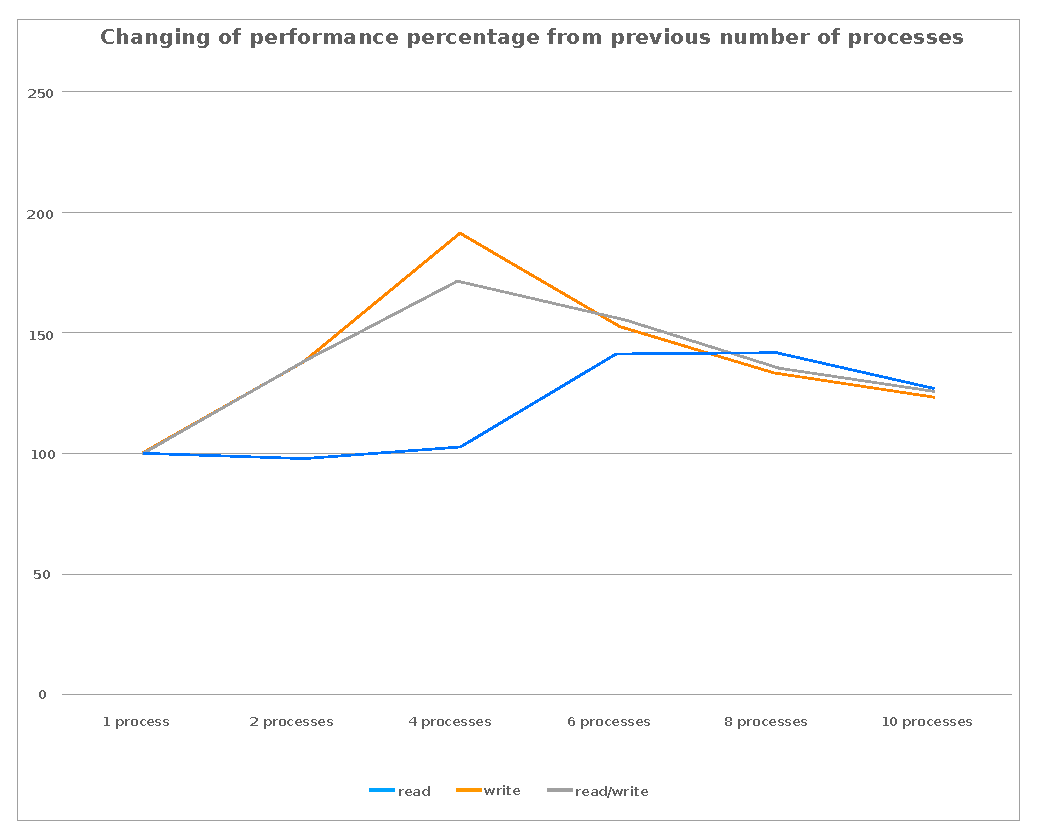
\includegraphics[scale=.7]{percentages.eps}
\end{figure}

\begin{figure}[H]
  \centering
  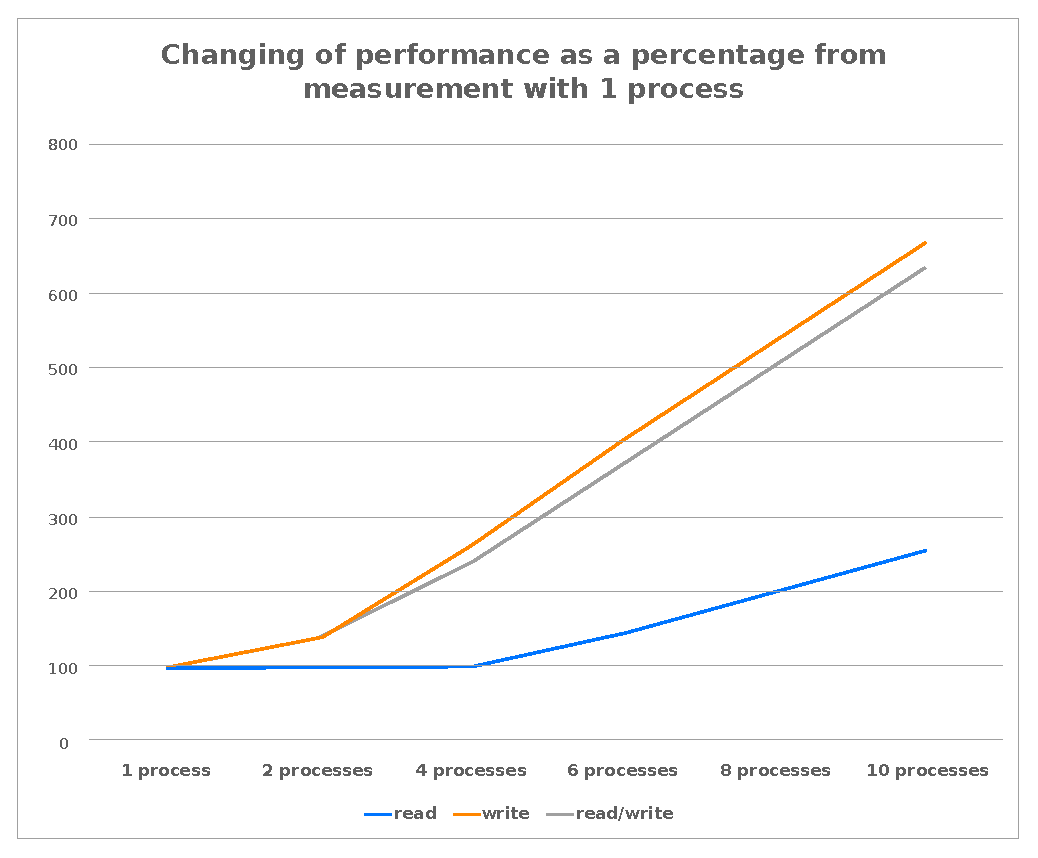
\includegraphics[scale=.6]{percentages1.eps}
\end{figure}

From plots we see that read operations much less expensive than write
operations. Reason of it is in that read operations look-up values only from RAM
and don’t make any work with storage instead of write operations.

From the last plot we can understand that behaviour of performance of write and
read/write operations can be explained as O(n) where n - number of processes
because growth of time of write and read/write operations increasing linearly
which is quite good in general.

But there are not differences between write and read/write operations what can
be explained by the reason that we couldn’t use read write semaphore or read
write spinlock.

\section{Discussion}
Developing for the Linux kernel was not an easy task. Much of the information
available online is outdated and the kernel in many places, is poorly
documented. Most of the time spent on the project, was dedicated to sifting
through kernel code, trying to to figure out what the functions do, which
functions to use and in what contexts they were safe to use.

Debugging was also difficult, in part because many debug tools run only in
user-space. Another complicating factor, was the fact that the operating
system could freeze when there was a bug in the code and that the error
print-outs were lost when rebooting.

Overall though, this was a very interesting project. It gave lots of insights
into the Linux kernel and forced you to get into the habit of reading and
trying to understand code, written by other people, perhaps less inclined to
properly document their work.

\end{document}
